\documentclass[12pt]{article}

\usepackage[margin=1in]{geometry}
\usepackage{amsmath,amsthm,amssymb}
\usepackage{mathrsfs}
\usepackage{mathtools}
\usepackage{enumitem}
\usepackage{physics}
\usepackage{pdfpages}

\newcommand{\magsq}[1]{\big|#1\big|^2}
\newcommand{\avg}[1]{\left<#1\right>}

\begin{document}
	
\title{Homework 5}
\author{Sean Ericson \\ Phys 684}
\maketitle

\section*{Problem 1}
Starting with the Maxwell wave equation

\section*{Problem 2}
In the steady state, the OBE are    
\[
\begin{rcases*}
0 =& $-\gamma u(t) - \delta v(t)$ \\
0 =& $\delta u(t) - \gamma v(t) - \Omega_0 w(t)$ \\
0 =& $-\gamma_2 (w(t) + 1) + \frac{\Omega_0}{2}v(t)$
\end{rcases*}
\implies
\mqty(-\gamma&-\delta&0\\\delta&-\gamma&-\Omega_0\\0&\Omega_0/2&-\gamma)\mqty(u\\v\\w) = \mqty(0\\0\\\gamma_2)
\]

\section*{Problem 3}
\begin{enumerate}[label=(\alph*)]
    \item 
\end{enumerate}

\section*{Problem 4}
\begin{enumerate}[label=(\alph*)]
    \item 
\end{enumerate}

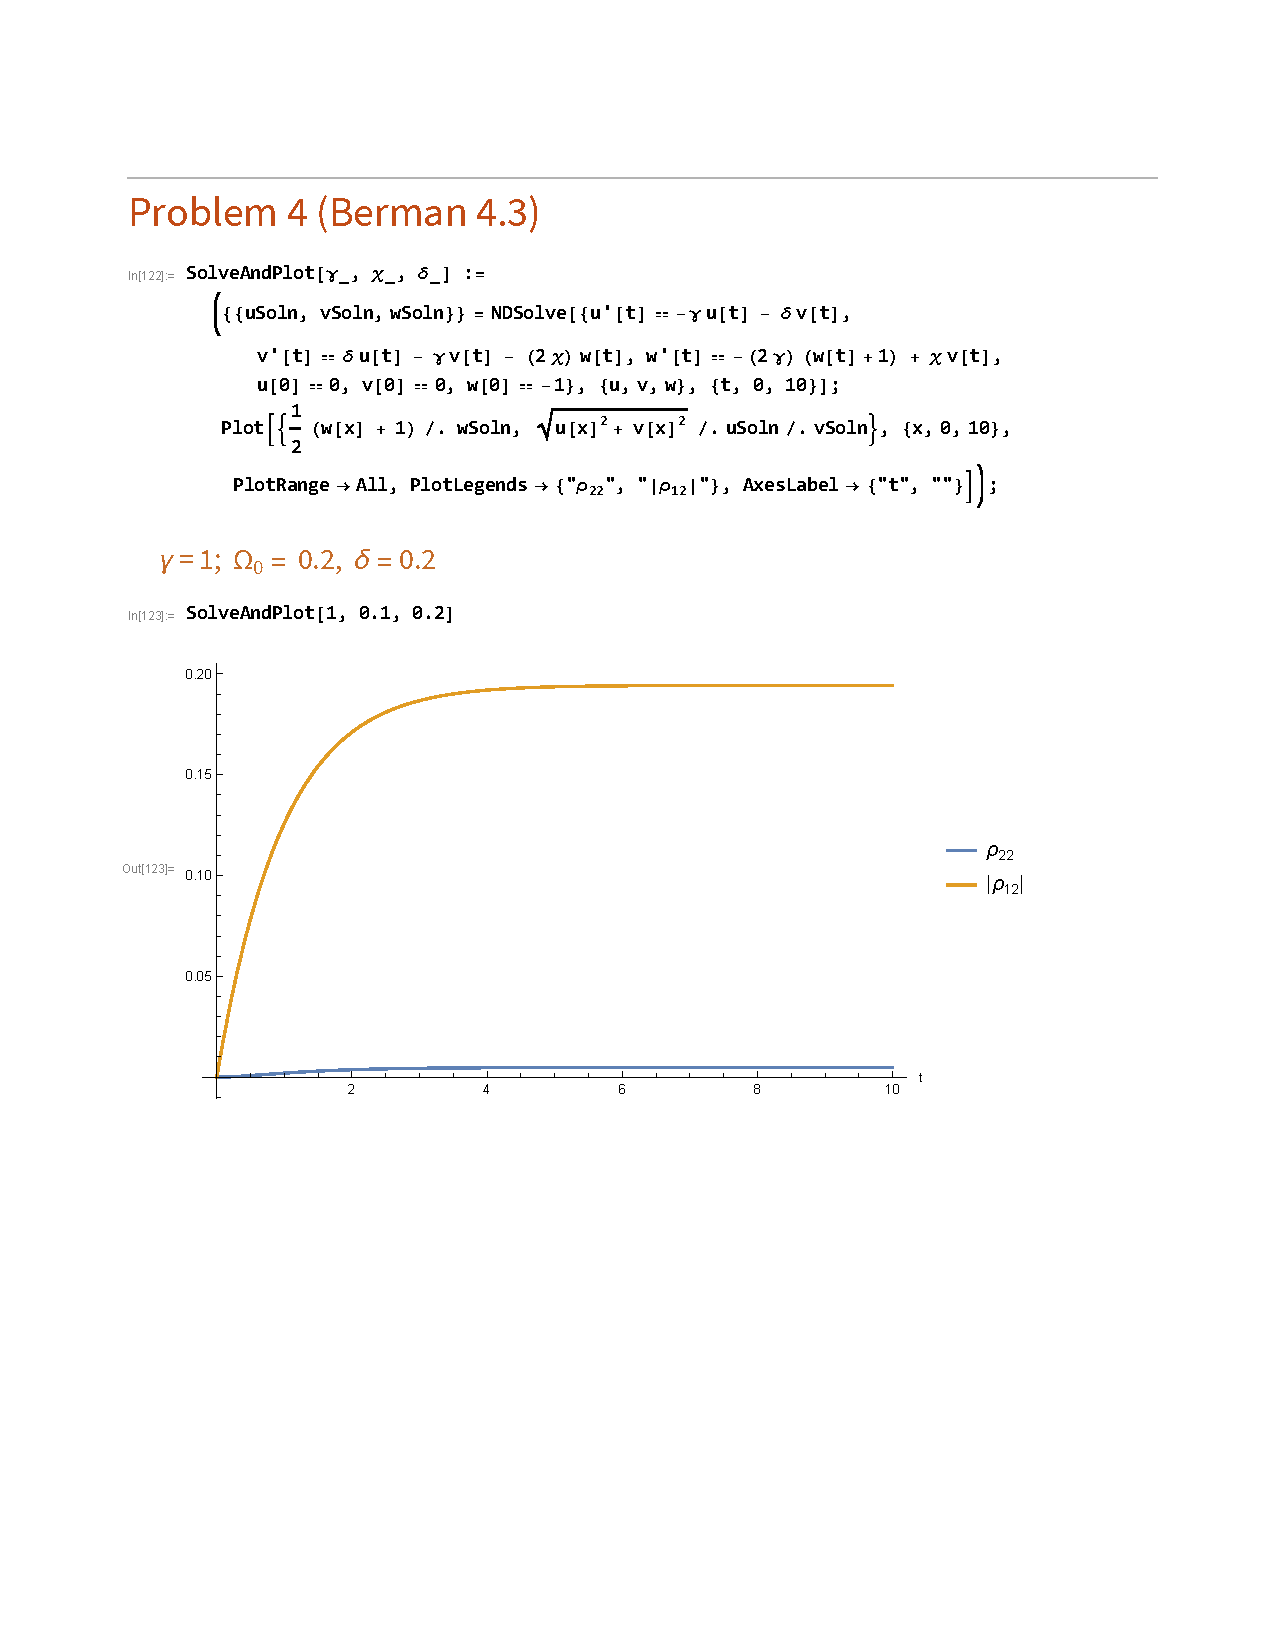
\includepdf[pages=-]{calcs/HW5_mathematica.pdf}
\end{document}